To prove the functional correctness of graph-manipulating algorithms implemented in a real language, we need to connect the heap representation of graphs, the memory model of the programming language, and the mathematical properties of graphs from \S\ref{sec:mathgraph}.  The first of these turns out to be surprisingly subtle as we shall see in \S\ref{sec:fixpointfail} and \S\ref{sec:goodgraph}.  The main challenge for the others is to engineer a framework that is generic enough and modular enough to be useful in practice in a variety of settings; we cover it in~\S\ref{sec:ramifylib}.

\subsection{Recursive definitions yield poor \p{graph} predicates}\label{sec:fixpointfail}

\newcommand{\graphkt}{\p{graph}_T}
\newcommand{\grapham}{\p{graph}_A}

Recursive predicates are ubiquitous in separation logic---so
much so that when a person writes the definition of a predicate as
\mbox{$P$ ``$\defeq$'' $\ldots P \! \ldots$}, no one raises an eyebrow despite the
dangers of circularity in mathematics. Indeed, the vast majority of the time there
is no danger thanks to the magic of the Knaster-Tarski fixpoint
$\mu_{\mathsf{T}}$ \cite{tarski:fixpoint}.  Formally what is going on
is instead of defining $P$ directly, one defines a functional
\mbox{$F_P \defeq \lambda P.~ \ldots P \! \ldots$} and then defines $P$ itself as
\mbox{$P \defeq \mu_{\mathsf{T}} \, F_P$}.  Assuming (as one typically does
without comment) that $F_P$ is \emph{covariant}, i.e. $(P \vdash Q)
\Rightarrow (F \, P \vdash F \, Q)$, one then enjoys the fixpoint
equation $P \Leftrightarrow \ldots P \ldots$, formally justifying
typically written pseudodefinition (``$\defeq$'').

%Definition corec {B A: Type}  (F: (B -> pred A) -> (B -> pred A)) : B -> pred A :=
%fun x w => forall P: B -> pred A, (forall x, F P x |-- P x) -> P x w.

Suppose we define a graph predicate $\graphkt$ this way, \emph{e.g.} along the lines of the fold/unfold definition in Figure~\ref{fig:markgraph}: %, \emph{i.e.}
\vspace{-1ex}
\[
\begin{array}{@{}l@{}l@{}}
\graphkt(x, \gamma) \stackrel{\Delta}{=} & (x = 0 /| \p{emp}) |/ \null \\
& \exists m,l,r.~ \gamma(x)=(m,l,r) /| \null \\
& ~~  x |-> m,l,r ** \graphkt(l, \gamma) ** \graphkt(r, \gamma)
\end{array}
\vspace{-1ex}
\]
%We have removed the alignment-related portions of equation~\eqref{eqn:bigraphintrofoldunfold} to focus on a more serious issue, even though as we will explain in~\S\ref{sec:goodgraph} alignment concerns are also necessary for the fold/unfold relationship to hold in C-like memory models.
The functional needed to define $\graphkt$ is covariant, so we can apply Knaster-Tarski; however, the result is hard to use.

Consider the following memory $m$ for a toy machine:

\begin{minipage}{.24\textwidth}
\qquad \[
\begin{array}{l|l}
\textrm{address} & \textrm{value} \\
\hline
102 & 0 \\
101 & 100 \\
100 & 42 \\
\end{array}
\]
\end{minipage}
\begin{minipage}{.19\textwidth}
\centering
\beginpgfgraphicnamed{selfref}
\begin{tikzpicture}
[->/.style={thick,arrows={-Stealth}},
   propG/.style={shape=circle, draw}]
   \path[use as bounding box] (-1, -1) rectangle (0.5, 0.5);
   \node[propG] (P) at (0, 0) {42};
   \draw[->] (P.west) .. controls (-1.5, 0) and (0, -1.5) .. (P.south);
\end{tikzpicture}
\endpgfgraphicnamed
\end{minipage}
\vspace{0.75ex}

\noindent Clearly $m |= 100 |-> 42,100,0$.  But it seems also clear that this memory represents a one-cell cyclic graph as illustrated in the accompanying diagram, \emph{i.e.} we want $m |= \graphkt(100,\hat{\gamma})$, where $\hat{\gamma}(100) = (42,100,0)$.  This is equivalent to wanting to be able to prove $100 |-> 42,100,0 |- \graphkt(100,\hat{\gamma})$.  Unfortunately, as hinted in Appendix~C\hide{\ref{apx:problemrecgraph}}, this seems rather difficult to do so since applying the natural proof techniques actually strengthen the goal.  In fact we do not know if this entailment is provable or not, but the difficulties encountered in proving what ``should be'' straightforward suggest that Knaster-Tarski should be treated with caution when defining spatial predicates for graphs.

The other direction, \mbox{$\graphkt(100,\hat{\gamma}) |- 100 |-> 42,100,0$},
\textbf{is} true but is not easy to prove, relying on the constructions in \S\ref{sec:goodgraph} and the fact that $\mu_{\mathsf{T}}$ constructs the least fixpoint.  In contrast, $\graphkt(100,\hat{\gamma}) |- 100 |-> 42,100,0 * \top$ is easy. % to prove. % via fold/unfold.

%As explained in~\S\ref{sec:foldunfold}, this alignment is necessary in C-like memory models to prove fold-unfold \eqref{eqn:bigraphintrofoldunfold}, which is why \eqref{eqn:bigraphintrofoldunfold} includes an alignment restriction $x~\mathsf{mod}~16 = 0$ and an existentially-quantified ``blank'' second field for the root $x \mapsto m,-,l,r$.

%As shown in (\ref{eqn:bigraphintrofoldunfold}) of Section
%\ref{sec:orientation}, Hobor and Villard\cite{hobor:ramification}
%defined the separation logic graph predicate
%$\mathsf{graph}(x,\gamma)$ in direct analogy to the standard
%separation logic definition of a tree. Note that the two-neighborhood
%means $\gamma$ is a BiGraph. However, it is peculiarly challenging in
%rigorously formalizing $\p{graph}$.

%* Showing that neither traditional fixpoint method works

%Appel and McAllester proposed another fixpoint $\mu_{\mathsf{A}}$
%that is sometimes used to define recursive predicates in separation
%logic \cite{appel:fixpoint}.  This time the functional $F_P$ needs to be
%\emph{contractive}, which to a first order of approximation means that
%all recursion needs to be guarded by the ``approximation
%modality''~$\rhd$~\cite{appel:vmm}, \emph{i.e.} our graph predicate would
%look like
%\begin{align*}
%\grapham(x, \gamma) ~ &\stackrel{\Delta}{=}\\
% (x = 0 /| \p{emp}) & |/ \exists m,l,r.~ \gamma(x)=(m,l,r) /| \null \\
% x |-> m,l,r & ** \rhd \grapham(l, \gamma) ** \rhd \grapham(r, \gamma)
%\end{align*}
%
%Unfortunately, $\rhd P$ is not precise for all $P$, so $\grapham$ is not precise either.  The approximation modality's universal imprecision has never been noticed before. % in the literature.  %We must do better.

%%%%%%%%%%%%%%%%%%%%%%%%%%%%%%%%%%%%%%%%%%%%%%%%%%
%%%%%% Edit0: cut down contractive recursion
%%%%%%%%%%%%%%%%%%%%%%%%%%%%%%%%%%%%%%%%%%%%%%%%%%

\subsection{Defining a good \p{graph} predicate}\label{sec:goodgraph}

Rather than trying to define \p{graph} as a recursive fixpoint, we will instead give it a flat structure.  Graphs in separation logic have been defined in similar ways before~\cite{ilya-graphs}; what is new here is that we prove---with the amount of precision required to convince Coq---that we can still enjoy fold/unfold with our definition.  Our path starts with the iterated separating conjunction or ``big star'', defined as:
%%%%%%%%%%%%%%%%%%%%%%%%%%%%%%%%%%%%%%%%%%%%%%%%%%
%%%%%% Edit1
%%%%%%%%%%%%%%%%%%%%%%%%%%%%%%%%%%%%%%%%%%%%%%%%%%
%%%%%% Edit1: Qinxiang's proposal starts
%%%%%%%%%%%%%%%%%%%%%%%%%%%%%%%%%%%%%%%%%%%%%%%%%%
\iftrue
\[
\begin{array}{@{}l@{}}
\underset{\{l_1, l_2,\dots,l_n\}}{\bigstar}P ~~ \defeq ~~ P(l_1) *
  P(l_2) * \dots * P(l_n) \\
\underset{S}{\bigstar} P ~~ \defeq ~~ \exists L.~ (\p{NoDup}\ L) /| (\forall x.~ x\ \p{in}\ L <=> x \in S) /| \underset{L}{\bigstar}P
\end{array}
\]
Big star $\bigstar$ is first defined over a list and then extended to sets.  We are now ready to define a good \p{graph} predicate:
\fi
%%%%%%%%%%%%%%%%%%%%%%%%%%%%%%%%%%%%%%%%%%%%%%%%%%
%%%%%% Edit1: Qinxiang's proposal ends
%%%%%%%%%%%%%%%%%%%%%%%%%%%%%%%%%%%%%%%%%%%%%%%%%%
%%%%%% Edit1: Original version starts
%%%%%%%%%%%%%%%%%%%%%%%%%%%%%%%%%%%%%%%%%%%%%%%%%%
\iffalse
\begin{equation*}
  \underset{\{l_1, l_2,\dots,l_n\}}{\bigstar}P ~~ \defeq ~~ P(l_1) *
  P(l_2) * \dots * P(l_n).
\end{equation*}
Formally $\bigstar$ is defined over a list rather than a set and is parameterized by a predicate $P$.  It is natural to extend $\bigstar$ to a set $S$ with an existentially-quantified duplicate-free list~$L$:
\[
\underset{S}{\bigstar} P ~~ \defeq ~~ \exists L.~ (\p{NoDup}\ L) /| (\forall x.~ x\ \p{in}\ L <=> x \in S) /| \underset{L}{\bigstar}P
\]
We use the same $\bigstar$ notation since the concepts are similar, but the existential adds a little pain since we need to prove that all choices of $L$ yield equivalent predicates.

We are now ready to give a good \p{graph} predicate:
\fi
%%%%%%%%%%%%%%%%%%%%%%%%%%%%%%%%%%%%%%%%%%%%%%%%%%
%%%%%% Edit1: Original version ends
%%%%%%%%%%%%%%%%%%%%%%%%%%%%%%%%%%%%%%%%%%%%%%%%%%
\vspace{-1.5ex}
\begin{equation}\label{eqn:iter_def}
  \p{graph}(x, \gamma) ~~ \defeq ~~ \underset{v \in \mathit{reach}(\gamma, x)}{\bigstar} v\mapsto\gamma(v)
\vspace{-1.5ex}
\end{equation}
$\gamma$ is a GeneralGraph and ``$x |-> \gamma(x)$'' is a predicate that says how a single node fits in memory; in Figure~\ref{fig:markgraph} it was:
\[
\exists m,l,r.~\gamma(x) = (m,l,r) /| x |-> m,-,l,r /| x\ \p{mod}\ 16 = 0
\]
$\gamma$ need not be a bigraph, but \emph{e.g.} can have many edges.

Our definition of \p{graph} is flat in the sense that there is no obvious way to follow the link structure recursively.  Happily, we can recover a general recursive fold/unfold (if $x |-> \gamma(x)$ and the GeneralGraph have the necessary properties):
\vspace{-1ex}
\begin{equation}
\label{eqn:unfold_graph}
\hspace{-1em}\begin{array}{@{}lc@{\hspace{1pt}}c@{\hspace{1pt}}l@{}}
\p{graph}(x,\gamma)  <=>  x |-> \gamma(x) ** \big(\!\!\!\!\!\!\!\!\!\!\!\!\!\underset{n \in \p{neighbors}(\gamma,x)}{\raisebox{-0.3ex}{\resizebox{0.75em}{!}{$\scon$}} \hspace{-2.18ex} \bigcup}\!\!\!\!\!\!\!\!\!\!\!\! \p{graph}(\gamma,n) \big) \\
[2pt]
\text{~~~ where ~~ }\underset{l_1,\dots,l_n}{\raisebox{-0.3ex}{\resizebox{0.75em}{!}{$\scon$}}\hspace{-2.18ex} \bigcup} \! \! P  \defeq  P(l_1) ** \ldots ** P(l_n) \end{array}
\vspace{-1ex}
\end{equation}

The proof of the $<=$ direction requires care. The difficulty is that if two nodes $x |-> \gamma(x)$ and $x' |-> \gamma(x')$ are \emph{skewed}, \emph{i.e.} ``partially overlapping'' with some---but not all---of $x$'s memory cells shared with $x'$, then the $\bigstar$ on the left hand side cannot separate them.  To avoid skewing we require $x |-> \gamma(x)$ be \emph{alignable}.  A predicate $P$ is alignable when
\[
\forall x,y.~ \Big(P(x) ** P(y) |- \big(P(x) /| x = y\big) |/ \big(P(x) * P(y)\big)\Big)
\]
That is, either they are completely on top of one another or they do not interfere at all.  In a Java-like memory model such as in HIP/SLEEK this property is automatic because pointers in such a model always point to the root/beginning of an object.  In contrast, in a C-like memory model such as in VST/CompCert, this property is not automatic because pointers can point anywhere.  In such a model, alignment is most easily enforced by storing graph nodes at addresses that are multiples of an appropriate size (16 in Figure~\ref{fig:markgraph}).

Some of our VST proofs do not use fold/unfold, instead preferring to use the lemmas in~\S\ref{sec:ramifylib} directly.  On the other hand, for HIP/SLEEK fold/unfold is vital, and knowing that the recursive relationship holds produces a pleasant feeling.  We also prove fold/unfold lemma for DAGs in which we get a $*$ between the root and its $\medocon$-joined neighbors. % rather than the $**$ present in \eqref{eqn:unfold_graph}.

\subsection{Ramification Libraries}\label{sec:ramifylib}

\begin{figure}[htbp]
\centering
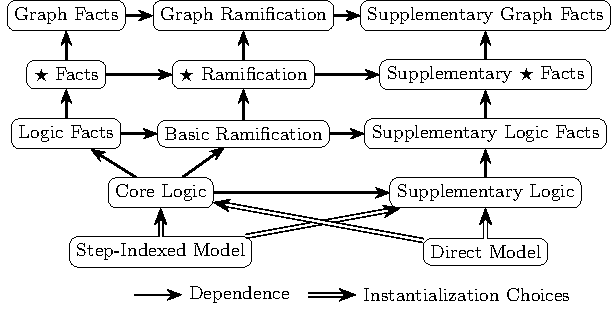
\includegraphics{infrastructure.pdf}
\caption{Infrastructure of ramification library}\label{fig:infra}
\end{figure}

We provide the architecture of our spatial development in Figure~\ref{fig:infra}.  Starting from the bottom, notice that there are two underlying heap models: the Step-Indexed Model, which is the main heap model used in VST, and a much simpler Direct Model, which is used by HIP/SLEEK among others.  The Step-Indexed model is much fancier, but none of our development depends on its bells and whistles.

To isolate our development from these unnecessary complications, and to ensure that HIP/SLEEK can reuse our spatial reasoning, we use two interfaces: Core Logic and Supplementary Logic.  Both models can instantiate both interfaces, but generally speaking our VST proofs only need the Core properties to prove our examples, whereas HIP/SLEEK uses both Core and Supplemental.  Each interface defines some operators of separation logic and provides some axioms about how they work.  For example, $*$ and $--*$ are in Core Logic, along with the axiom $(P |- Q --* R) <=> (P * Q |- R)$.  On the other hand, the $**$ and $--o$ operators are in Supplementary Logic, along with rules like $P |- P ** P$.

Above the Logic layer we have three towers, each three levels high.  The leftmost tower contains basic lemmas about Logic, $\bigstar$, and \p{graph}.  In the $\bigstar$ Facts box we prove \emph{e.g.}:
\[
\infrule{}
{A \cap B = \emptyset}
{\underset{x\in A}{\bigstar} P(x) *   \underset{x\in B}{\bigstar} P(x) \Leftrightarrow \underset{x\in A \cup B}{\bigstar} P(x)}{}
\]

The middle tower is more interesting in that it is entirely focused on ramification entailments.  A robust library of ramification entailments is essential to make ramification work smoothly in practice.  The lowest level contains lemmas like:
\[
%\infrule{Ramify-Q-SPLIT}
\infrule{}
{G_1 \vdash L_1 * \forall x.~ (L_2 --* G_2) \\
 G'_1 \vdash L'_1 * \forall x.~ (L_2' --* G'_2)}
{G_1 * G'_1 \vdash (L_1 * L'_1) * \forall x.~ \big((L_2 * L'_2)--* (G_2 * G'_2)\big)}{}
\]
We use this lemma to break large ramification entailments into more manageable pieces in a compositional way. % compositionally.

The middle level contains $\bigstar$ ramification lemmas, \emph{e.g.}:
\begin{equation}
\label{ramify:bigstar}
\infrule{}
{A \cap B = \emptyset  \qquad  A' \cap B = \emptyset}
{\underset{x\in A\cup B}{\bigstar} P(x) \vdash \! \underset{x\in A}{\bigstar} \! P(x) * \Big( \underset{x\in A'}{\bigstar} \! P(x) \! \wand \! \! \! \! \underset{x\in A' \cup B}{\bigstar} \! \! P(x)\Big)}{}
\end{equation}

The top level is focused on graph ramifications, such as the following ``update one node'' lemma:
\begin{equation}
\label{lem:updategraphnode}
%{\gamma(x_0) = \gamma'(x_0) \text{ for any } x_0 \neq x }
\infrule{}
{\forall x_0 \neq x.~ \gamma(x_0) = \gamma'(x_0) \\ \p{neighbors}(\gamma,x)=\p{neighbors}(\gamma',x)}
{\p{graph}(x, \gamma) \! \vdash \! x \! \mapsto \! \gamma(x) \! * \! \big(x \! \mapsto \! \gamma'(x) \! \wand \! \p{graph}(x, \gamma')\big)}{}
\end{equation}
This lemma was used on line~\ref{code:markram2} in Figure~\ref{fig:markgraph}.

This layered structure enables proof reuse. All of the theorems for $\p{graph}$ are proved from the properties of iterated separating conjunction, but having a modular library allows $\bigstar$ to be reused in other structures smoothly.

Also, all of our verifications of different graph algorithms use the proof rules of $\p{graph}$ at the top level in the library. Taking the marking algorithm we introduced in \S\ref{sec:orientation} as an example, we prove the following theorem from the library:
\begin{equation}
\label{lem:updatesubgraph}
\infrule{}
{n \in \p{neighbors}(\gamma,x)}
{
\mbox{
$\begin{array}{@{}l@{}l@{}}
\p{graph}(x, \gamma) \vdash \\
\p{graph}(n, \gamma) \! * \!
\big(\forall \gamma'. & \m{mark}(\gamma, n, \gamma') \! /| \! \p{graph}(n, \gamma') \! --* \null \\
& \m{mark}(\gamma, n, \gamma') \! /| \! \p{graph}(x, \gamma')\big)
\end{array}$
}
}{}
\end{equation}

The Supplementary tower contains properties not used by most of the VST examples.  This includes the fold/unfold relationship from \S\ref{sec:goodgraph}, facts about precision, and so forth.  Some of these properties are needed by HIP/SLEEK, while others are mostly included for esthetic effect.

% are there just because we felt they might be useful in the future.

%One benefit of the definition in (\ref{eqn:iter_def}) is that the pure
%mathematical graph $\gamma$ in $\mathtt{graph}$ is not necessarily a
%BiGraph. (\ref{eqn:iter_def}) can represent a general graph with
%variant number of neighors as long as extending the definition of
%$\gamma(x)$ to data mapped by the label function and every neighbor of
%node $x$.
%
%Moreover, it turns out that the $\bigstar$ notation is a more useful
%and fundamental concept than $\mathtt{graph}$. There are two parts of
%the $\bigstar$ in (\ref{eqn:iter_def}): one is the predicate $\mapsto$
%and the other is the node set which the $\mapsto$ iterates on. They
%both bind to $\gamma$ in (\ref{eqn:iter_def}) for $\p{graph}(x,
%\gamma)$, which is a special case. In section \ref{sec:applicable}, we
%will see the specification of a spanning tree algorithm which uses
%$\bigstar$ directly instead of $\p{graph}$ because in that
%specification, the predicate $\mapsto$ and the node set bind to
%different mathematical graphs. Furthermore, we generalize the
%ramification rules for $\p{graph}$ in \cite{hobor:ramification}, which
%uses $\bigstar$ so as to be applied in all verification examples.

%% 1.2. \texttt{Iter\_sepcon} and \texttt{pred\_sepcon} are defined. And related ramification rules are proved.
%% 1.3. The most general graph-spatial-predicate \texttt{vertices\_at} are defined (for all possible styles of graphs). Related ramification rules are proved. Graph and graphs are defined as special cases of vertices at.

%% 2. A minor implementation trick. There are many tactics defined in \texttt{msl\_ext/ramify\_tactics.v}, which can manipulate low level heaps efficiently.

%% * Separating the material into the general vs. tool-specific part.  Measurements of etc.
